%! TEX root = **/000-main.tex
% vim: spell spelllang=en:

\subsection{Normalized arcsine kernel}

\subsubsection{Regression}

\Cref{fig:nrmse-asinnorm-scaled} shows the obtained normalized root mean
squared error (nRMSE) for each dataset and each value of $\sigma$ for all the
regression kernels tested using the normalized arcsine kernel. We show the
\emph{nRMSE} for the best combination (the one with minimal \emph{nRMSE})
of the other hyperparameters ($C$ and $\varepsilon$) for each value of sigma.
The value for \emph{nRMSE} is the mean of the 10 folds and the shaded area
represents the 95\% confidence interval.
As a reference, we present the best results obtained by the radial basis
function (RBF) kernel as a dashed horizontal line with its corresponding
95\% confidence interval as dotted lines.

\begin{figure}[H]
    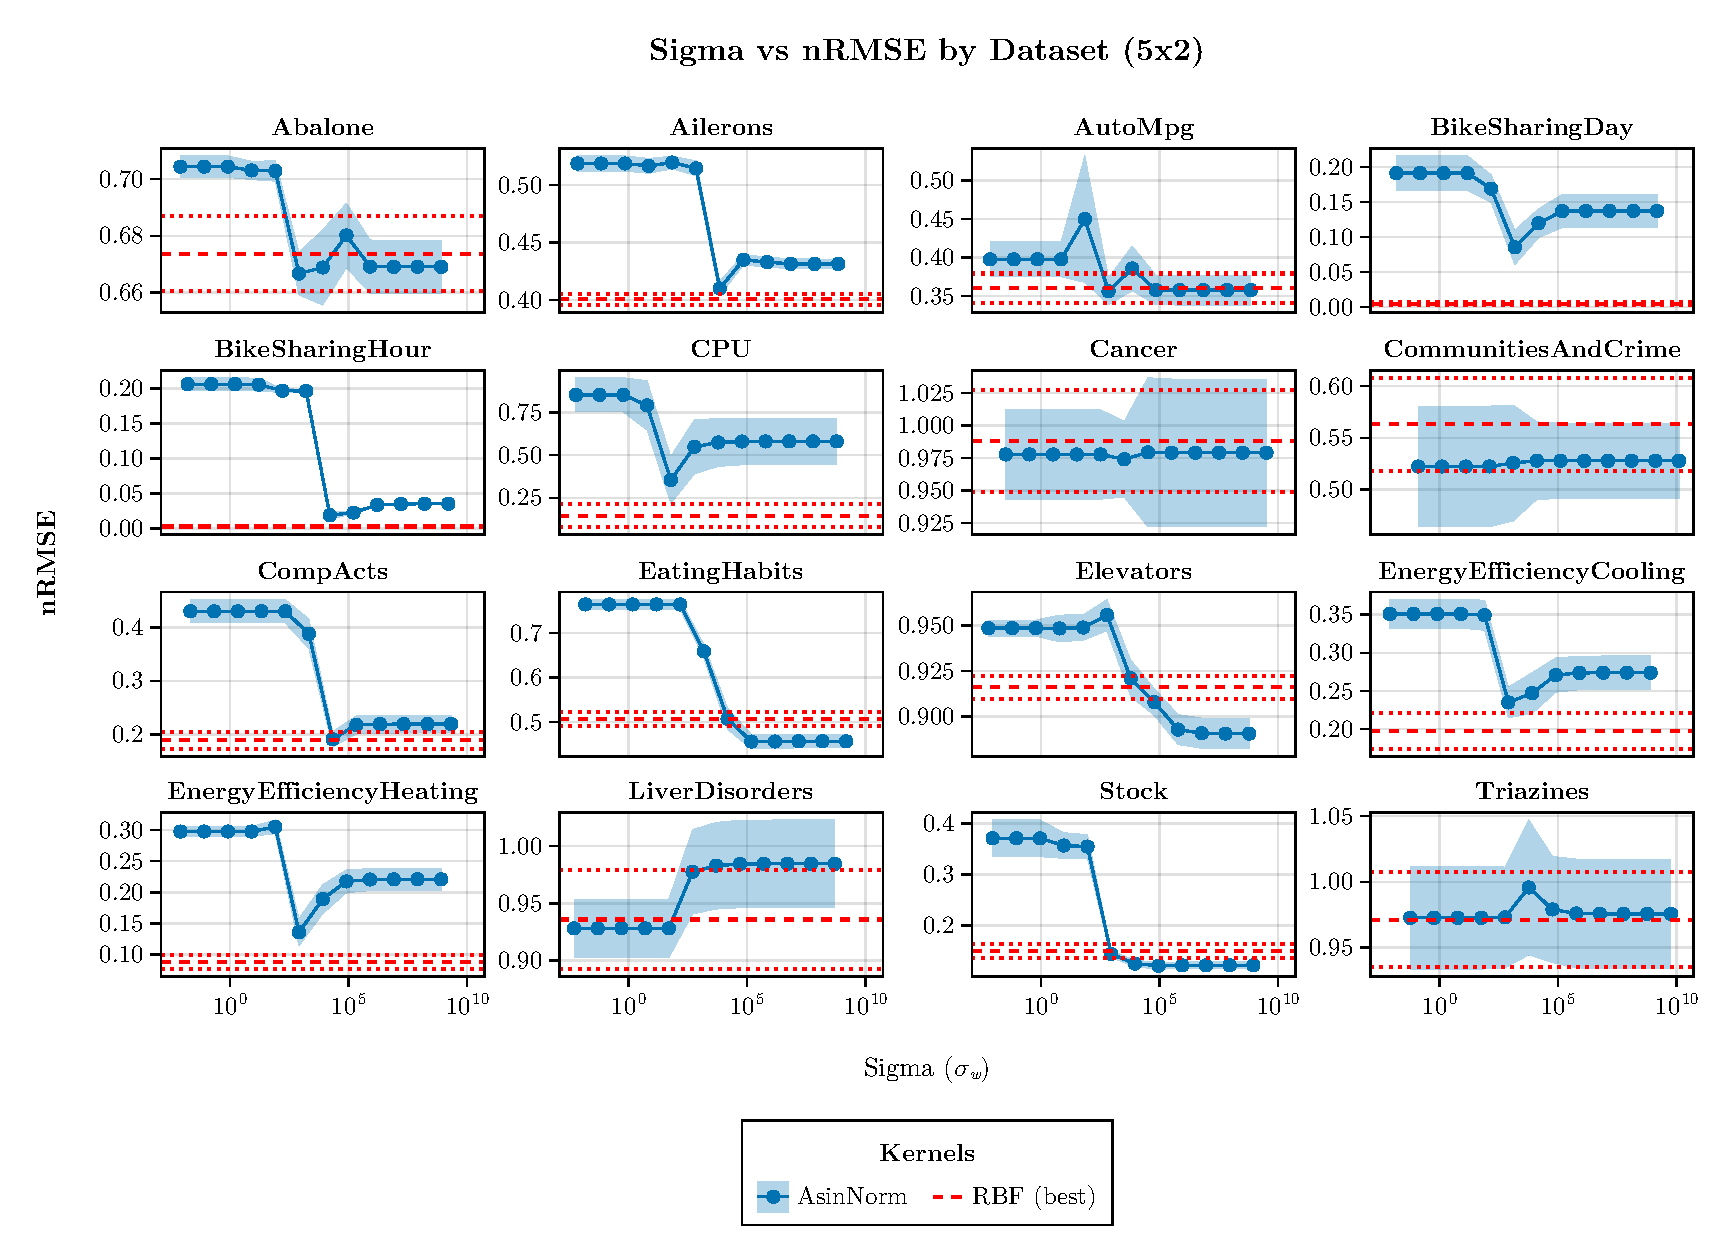
\includegraphics[width=\textwidth]{plots/nRMSE_nodelve_asinnorm_scaled_unlinked}
    \caption{Sigma vs Normalized Root Mean Squared error by dataset using Normalized arcsine kernel}%
    \label{fig:nrmse-asinnorm-scaled}
\end{figure}

From this figure we can observe some interesting results:

\begin{enumerate}
    \item Except for \texttt{BikeSharingDay} and \texttt{EnergyEfficiencyHeating},
          the normalized arcsine kernel has at least one point in which the \emph{nRMSE} is
          within the confidence interval of the RBF kernel.
    \item The kernel seems to stabilize for $\sigma \geq 10^5$. This supports
          the idea of the kernel being insensitive to the value of $\sigma$.
    \item In some cases, the normalized arcsine kernel outperforms \emph{RBF}:
          \texttt{EatingHabits}, \texttt{Elevators} and \texttt{Stock}.
    \item Looking at \texttt{Ailerons} we see that for a specific value of
          $\sigma$, the results are similar to the RBF kernel, but deviating
          from that value increases the \emph{nRMSE} significantly. This can also
          be observed in \texttt{BikeSharingHour}, \texttt{CompActs} and \texttt{EnergyEfficiencyCooling}.
\end{enumerate}

These observations hint that the kernel, although it may stabilize to the same
performance for high values of sigma, this high values of sigma may not be
optimal.

If we now look at the results for the \texttt{Delve} datasets shown in
\cref{fig:nrmse-delve-asinnorm-scaled}. In the figure, we show the results for
all 8 combinations of features (8 or 32), linearity (fairly linear or nonlinear)
and noise (moderate or high) for each of the two synthetic datasets. This
gives a total of 16 datasets.

From the Delve datasets we can further observe:
\begin{enumerate}
    \item The arcsine kernel struggles (does not reach parity with the results from RBF)
          with the Bank dataset with 32 features and moderate noise in
          both fairly linear and nonlinear cases.
    \item We observe the same pattern described in the previous plot for
          \texttt{Ailerons} in the \texttt{Delve} datasets. That is,
          there is a value of $\sigma$ which gives similar results to the RBF and
          deviating from that value increases the \emph{nRMSE}.
    \item In the high noise cases with 32 features (bottom right plot
          of each subdivision) the arcsine kernel behaves similarly to the RBF kernel
          or outperforms it (PumaDyn non-linear).
    \item In general, the best results for the arcsine kernel in relation to the
          RBF kernel are obtained in the combination of high noise and non-linear
          cases. Which are the ``hardest'' problems and arguably the ones which
          are more similar to real world problems.
\end{enumerate}

% \begin{figure}[H]
%     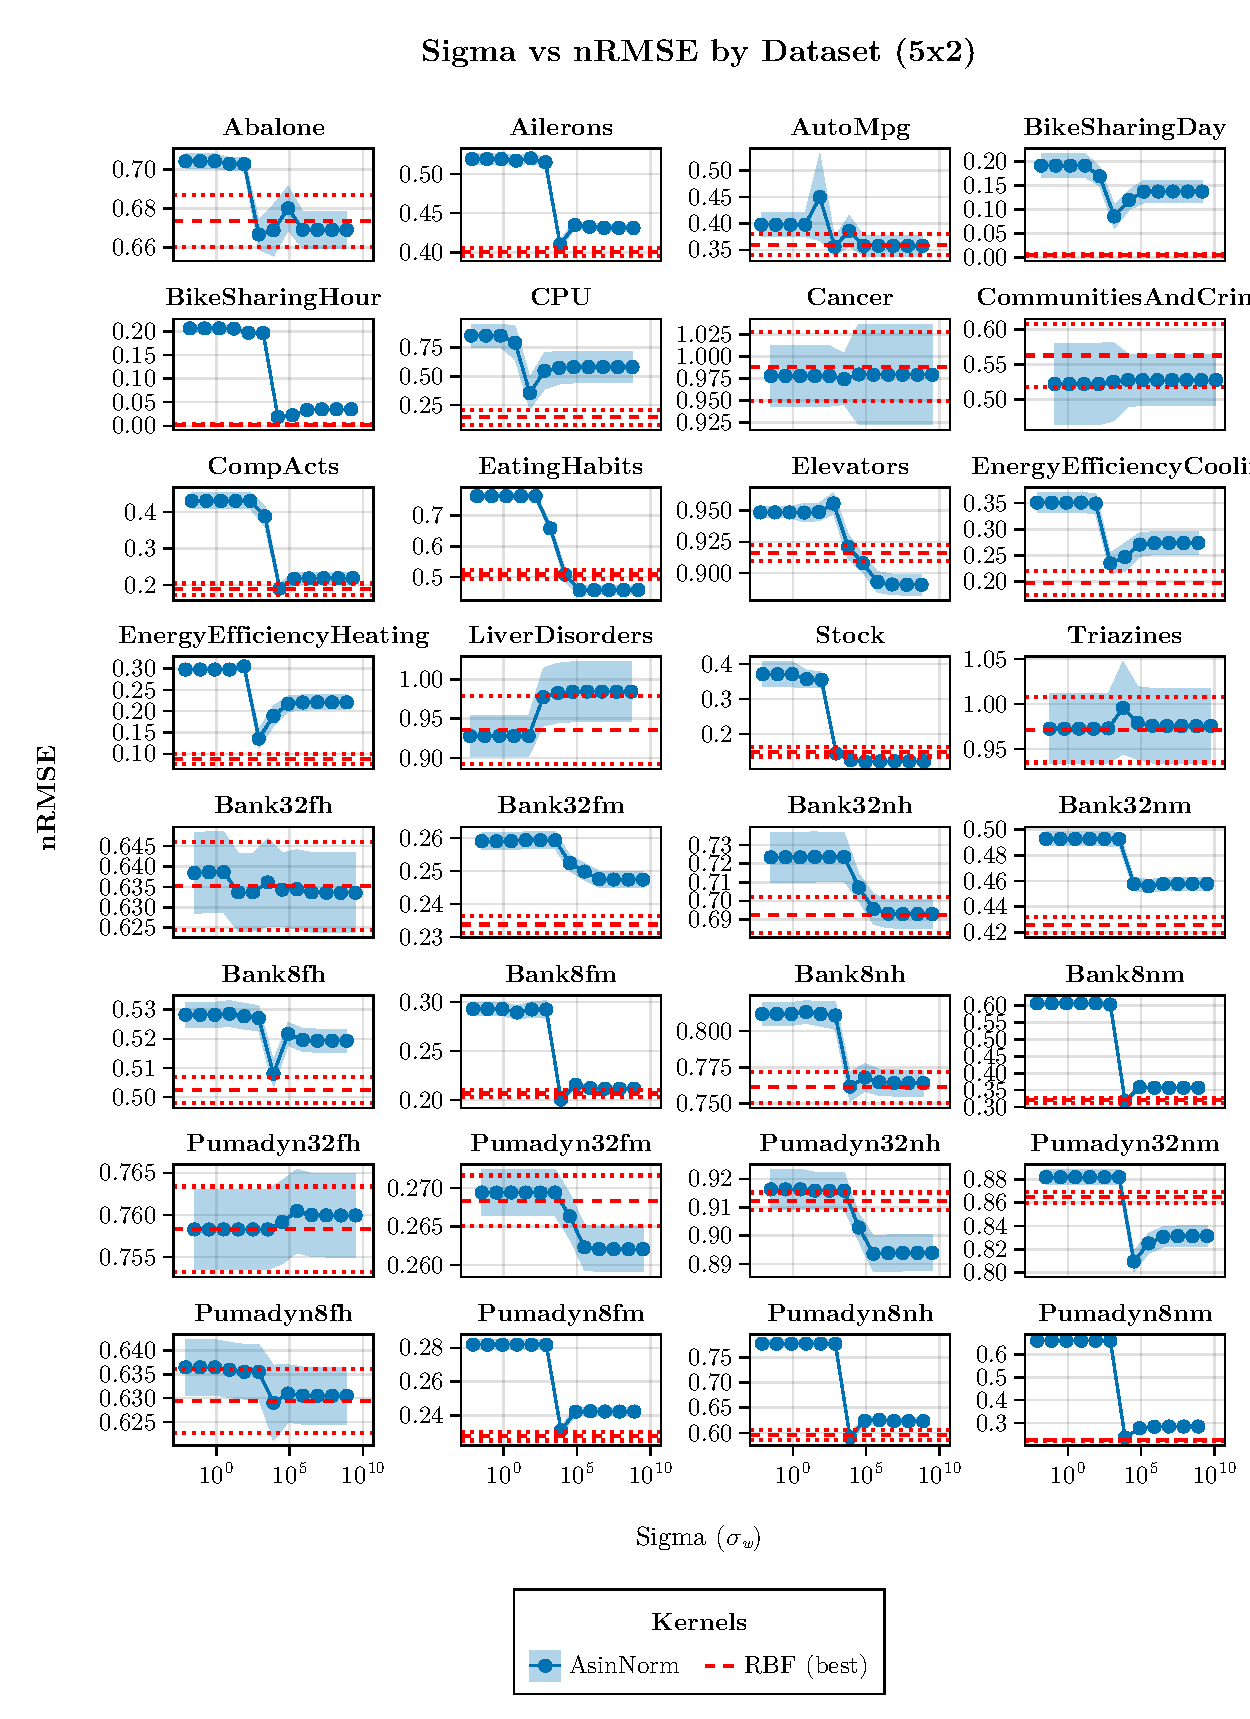
\includegraphics[width=\textwidth]{plots/nRMSE_asinnorm_scaled}
%     \caption{Sigma vs Normalized Root Mean Squared error by dataset using Normalized arcsine kernel}%
%     \label{fig:nrmse-asinnorm-scaled}
% \end{figure}

% \begin{figure}[H]
%     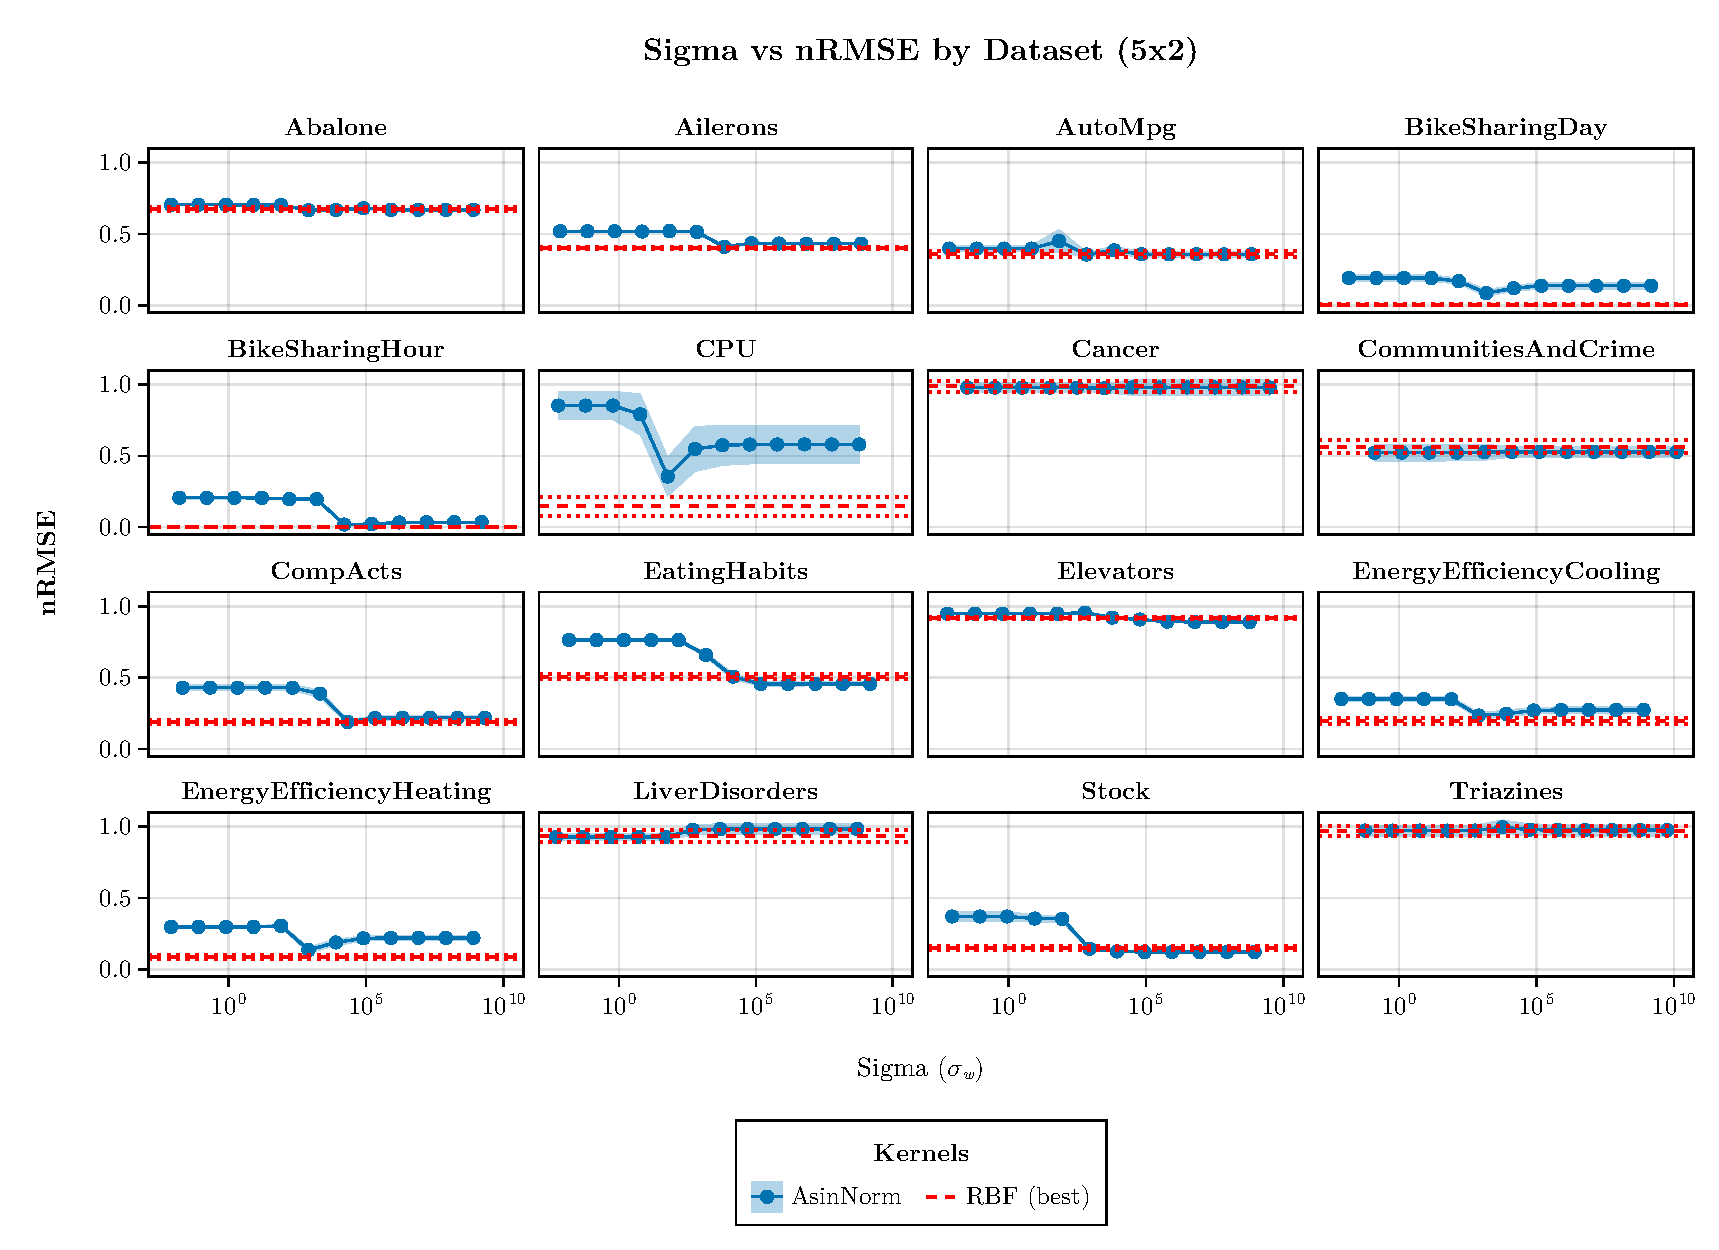
\includegraphics[width=\textwidth]{plots/nRMSE_nodelve_asinnorm_scaled}
%     \caption{Sigma vs Normalized Root Mean Squared error by dataset using Normalized arcsine kernel}%
%     \label{fig:nrmse-asinnorm-scaled}
% \end{figure}

% \begin{figure}[H]
%     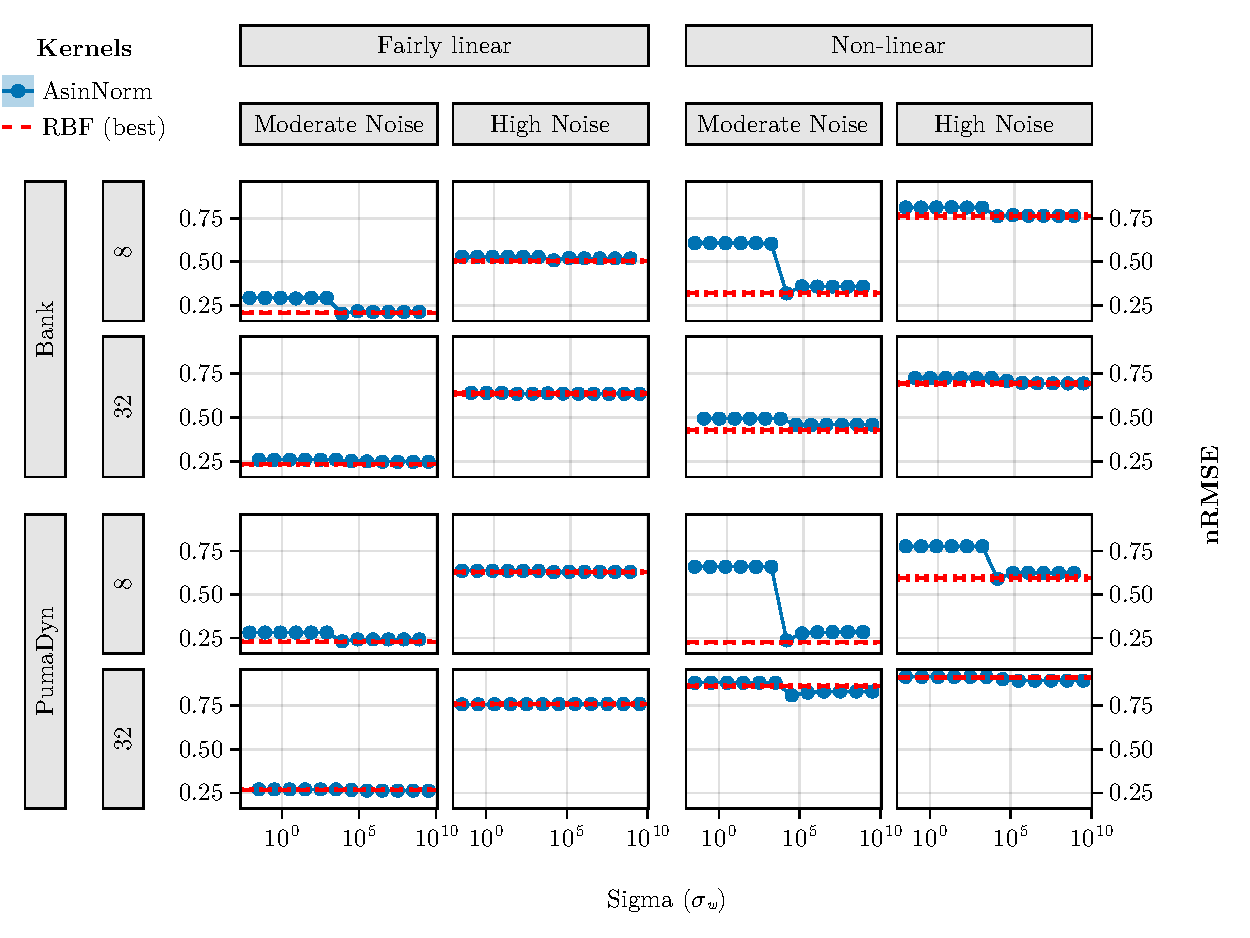
\includegraphics[width=\textwidth]{plots/nRMSE_delve_asinnorm_scaled}
%     \caption{Sigma vs Normalized Root Mean Squared error by dataset using Normalized arcsine kernel}%
%     \label{fig:nrmse-delve-asinnorm-scaled}
% \end{figure}

\begin{figure}[H]
    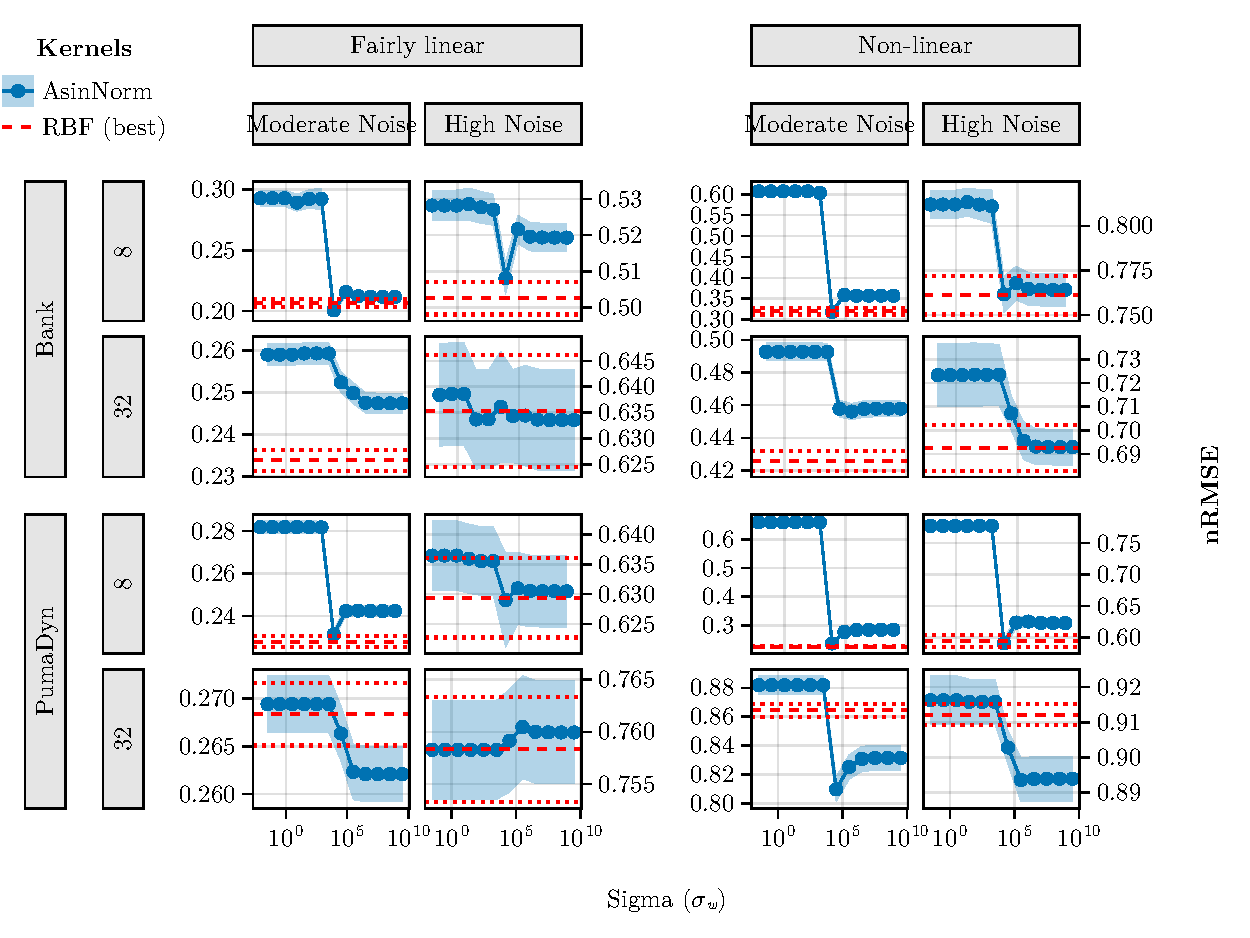
\includegraphics[width=\textwidth]{plots/nRMSE_delve_asinnorm_scaled_unlinked}
    \caption{Sigma vs Normalized Root Mean Squared error by dataset using Normalized arcsine kernel on
        Delve datasets}%
    \label{fig:nrmse-delve-asinnorm-scaled}
\end{figure}

\subsubsection{Classification}

\Cref{fig:accuracy-asinnorm-scaled} shows the obtained accuracy for each
of our classification datasets. Only \texttt{Adult} and \texttt{GlassIdentification}
differ from the results obtained by the RBF kernel. In the case of \texttt{Adult},
we can clearly see a point in which the accuracy reaches parity with the RBF
kernel. For $10^5$ it obtains the best accuracy and further increasing the sigma
stabilizes slightly below the RBF kernel (but inside the confidence interval). For
\texttt{GlassIdentification} there is a drop in accuracy with higher values of
sigma, which is not what we expected. A similar behaviour can be observed in
\texttt{Iris} to a lesser extent. It is unclear why this happens.

% TODO: glass why?

\begin{figure}[H]
    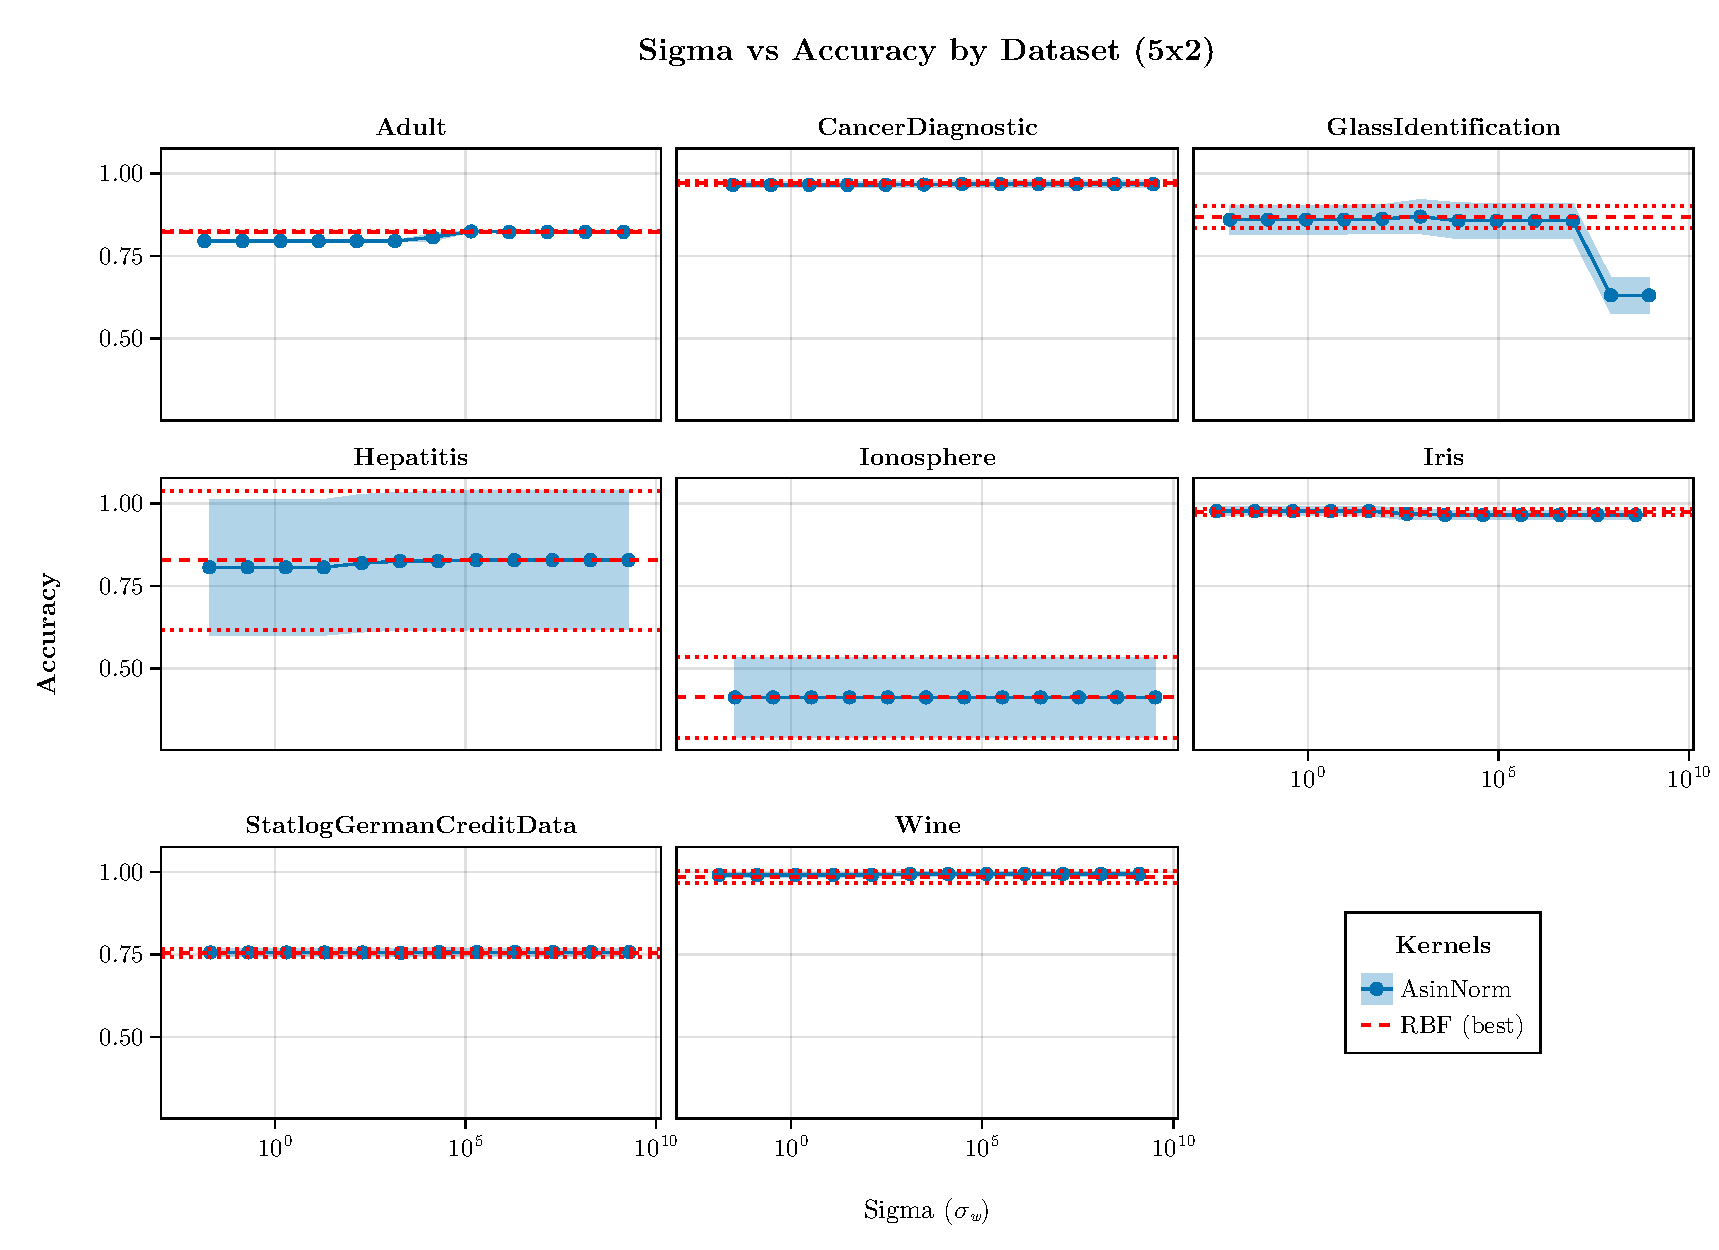
\includegraphics{plots/accuracy_class_asinnorm_scaled}
    \caption{Sigma vs Accuracy by dataset using Normalized arcsine kernel}%
    \label{fig:accuracy-asinnorm-scaled}
\end{figure}

\subsubsection{Comparison with radial basis (RBF) kernel}%
\label{ssub:comparison_with_radial_basis_rbf_kernel}

The statements made in the previous sections, hint that the normalized arcsine
kernel are based on observations of the different plots presented. However,
without some statistical analysis, we cannot draw any meaningful conclusions
beyond that. In this section, we will perform the paired t-test as described in
\cref{sec:paired-t-test} to assess whether the differences in performance which
we observe are statistically significant or are just anecdotal.


In particular, we are interested in how
the sigma parameter affects the performance of the kernel. For this reason,
we compare the different values of sigma for the arc-sine kernel against the
values of gamma for the RBF kernel.

For each dataset, $\sigma$ and $\gamma$ combination we perform a paired t-test
against the best combination of hyperparameters ($C$ and $\varepsilon$) for
each kernel. \Cref{fig:paired-ttest-rbf-asinnorm} shows the $p$\textendash{}values
obtained for these paired t-test results. The darker the color, the lower the
$p$\textendash{}value and the more significant the difference between the two
kernel configurations.

\begin{figure}[H]
    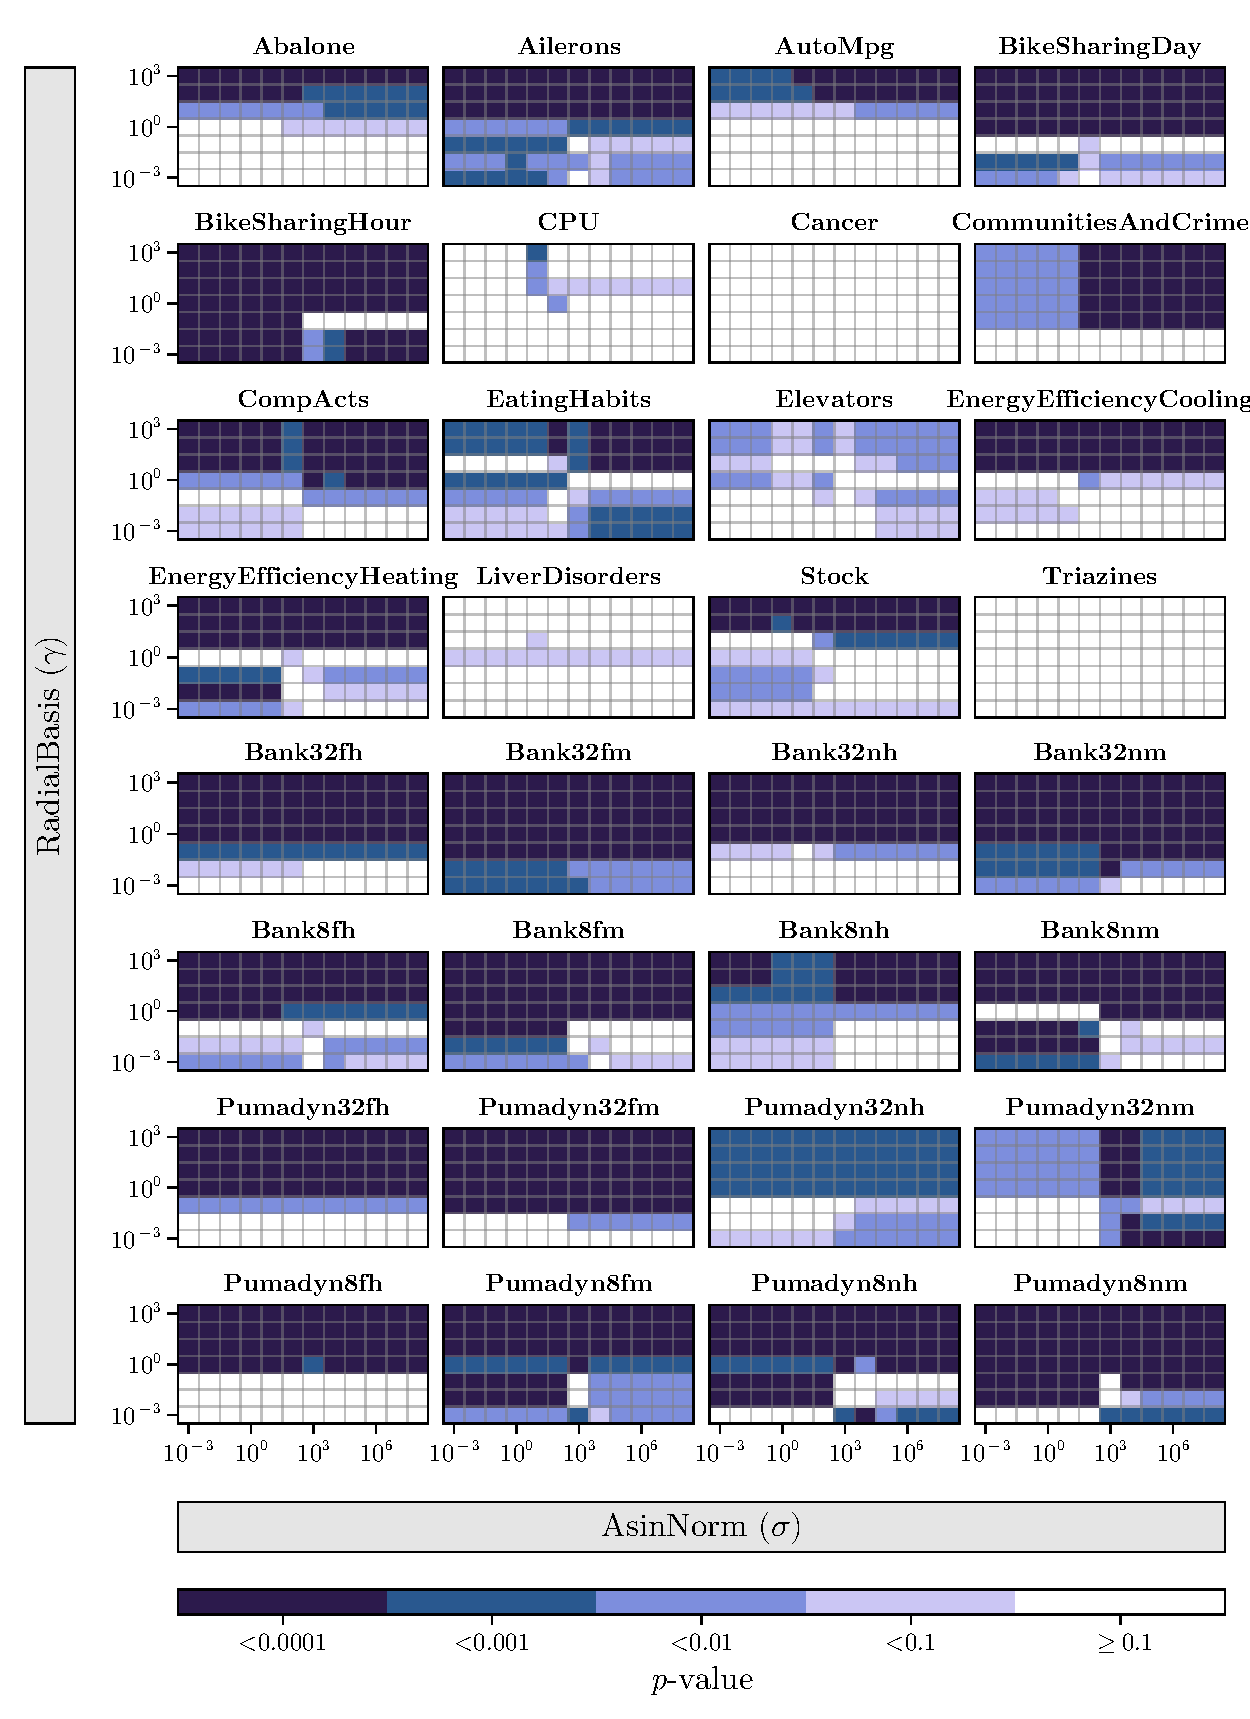
\includegraphics[width=0.9\textwidth]{plots/heatmaps_rbf_asinnorm_pvalues}
    \caption{p values}
    \label{fig:paired-ttest-rbf-asinnorm}
\end{figure}

From \cref{fig:paired-ttest-rbf-asinnorm} we can observe that:
\begin{enumerate}
    \item \texttt{Cancer}, \texttt{Triazines} \texttt{LiverDisorders}, and \texttt{Elevators} do not
          show significant differences between the kernels at any value of sigma or gamma.
    \item Other datasets such as \texttt{PumaDyn32fh} show no variation across the different
          values of sigma, which indicates that changing sigma has no effect on the
          relative performance of the kernel against the RBF kernel for those datasets.
\end{enumerate}

The patterns shown in the $p$\textendash{}values are not very useful since they
don't show the magnitude of the difference between the two kernels, nor do they
show the direction of the difference. For this reason, in \cref{fig:paired-ttest-rbf-asinnorm-diff}
we show the difference between the nRMSE of the RBF kernel and the normalized arcsine
kernel. The darker the color, the larger the difference between the two kernels. Red
values indicate that RBF performs better than the normalized arcsine kernel and blue
values indicate that the normalized arcsine kernel performs better than the RBF kernel.
All values that are outside the significance level $\alpha=0.001$ (that is, the
$p$\textendash{}value is higher than $\alpha$) have been removed and are shown as
white. Note that the $0$ in the colorscale is not pure white, but grey.

%  TODO: add pattern or something so the color can be seen in b/w
\begin{figure}[H]
    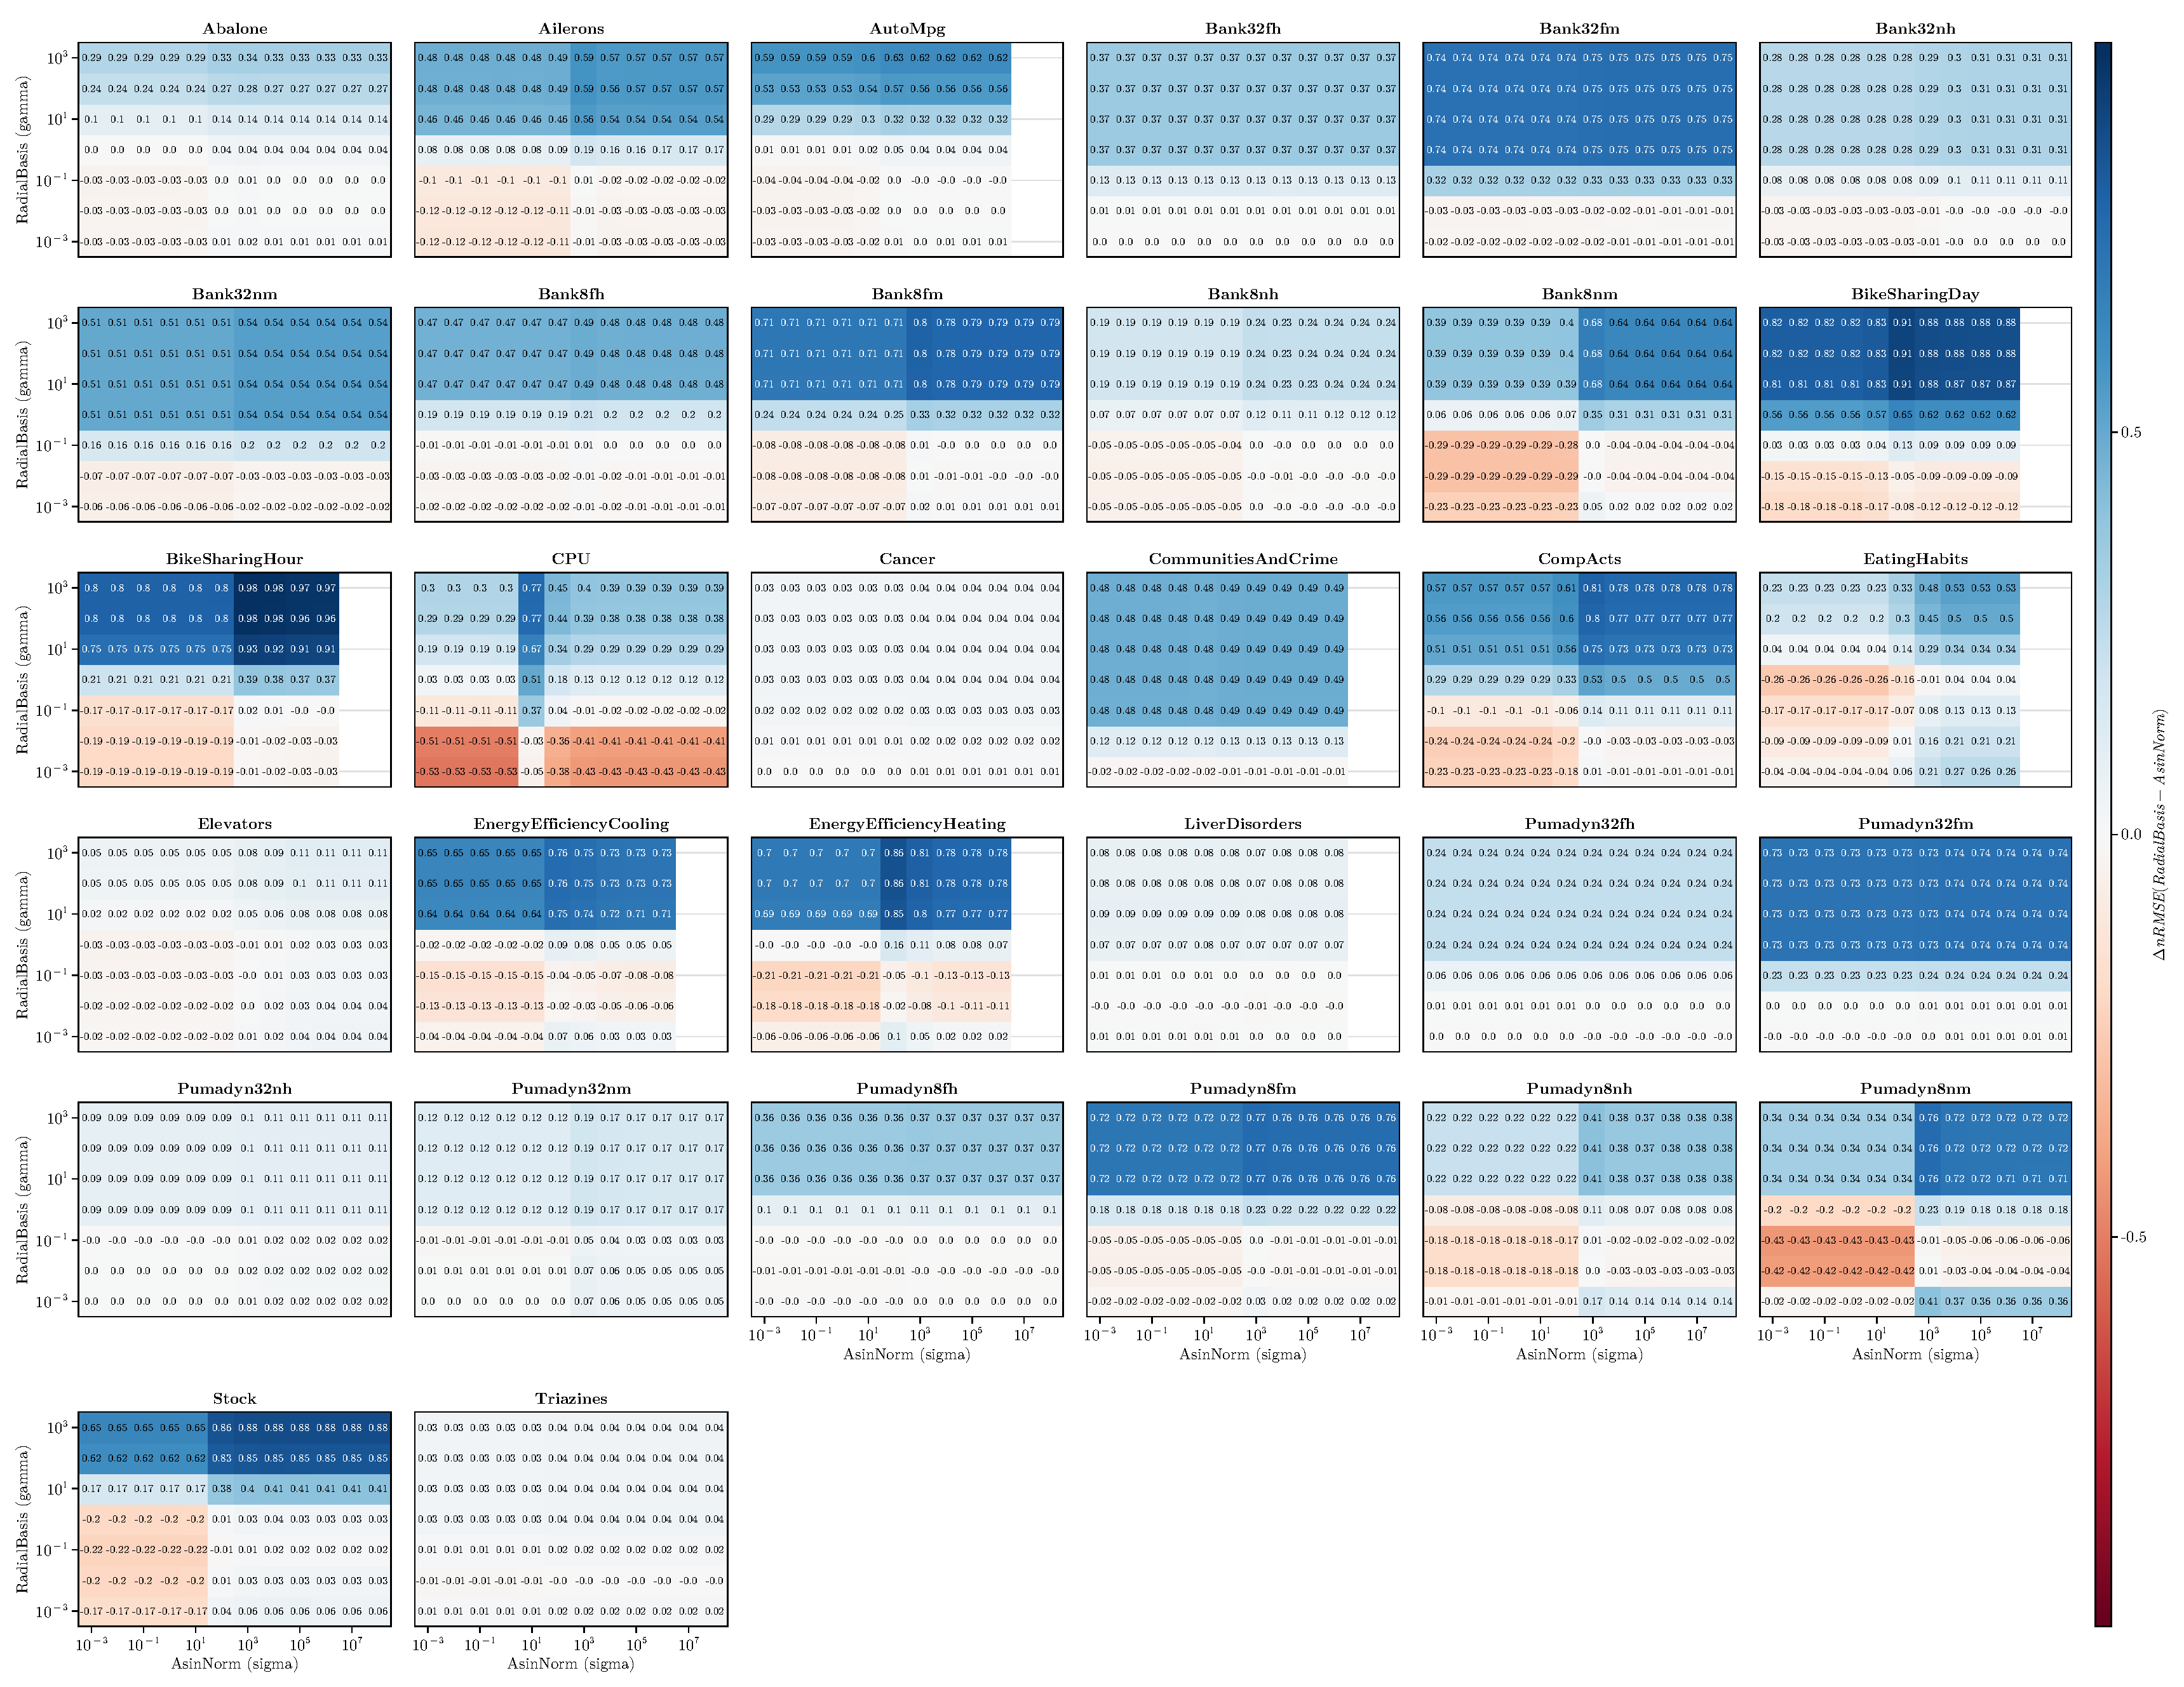
\includegraphics[width=0.9\textwidth]{plots/heatmaps_rbf_asinnorm}
    \caption{Difference between nRMSE of RBF and normalized arc-sine kernels ($\alpha=0.001$)}
    \label{fig:paired-ttest-rbf-asinnorm-diff}
\end{figure}

The way we interpret \cref{fig:paired-ttest-rbf-asinnorm-diff} is based on whether
we can see a value of sigma in which all the values to its right are blue or white.
Meaning that the normalized arcsine kernel performs better (blue) or there is no
statistically significant difference (white). All datasets except
\texttt{PumaDyn8nm} and \texttt{BikeSharingHour} show this behaviour.

In both \texttt{PumaDyn8nm} and \texttt{BikeSharingHour} we can see that all
differences for $\sigma=10^3$, are either positive (favoring the Asin kernel) or
not statistically significant, whilst for values higher there is a mix of positive
and negative values. This indicates that for $10^3$ the normalized arcsine kernel
reaches parity with the RBF kernel and for higher values of sigma, the performance
of the normalized arcsine kernel is not as good as the RBF kernel. Looking
at the previous plots (\cref{fig:nrmse-asinnorm-scaled,fig:nrmse-delve-asinnorm-scaled})
we can see that this is one of the cases in which we described the behaviour of
an ``optimal'' value of sigma which loses performance in both directions.

\subsubsection{Computational Cost}

It is difficult to compare the computational cost between the RBF kernel
and the normalized arcsine kernel. Since their performance is dependent
on the parameter selection and the dataset. \Cref{fig:time-asinnorm-scaled-compacts}
shows the boxplots of all executions of the normalized arcsine and rbf kernels
on the \texttt{CompActs} dataset grouped by the cost hyperparameter.

\begin{figure}[H]
    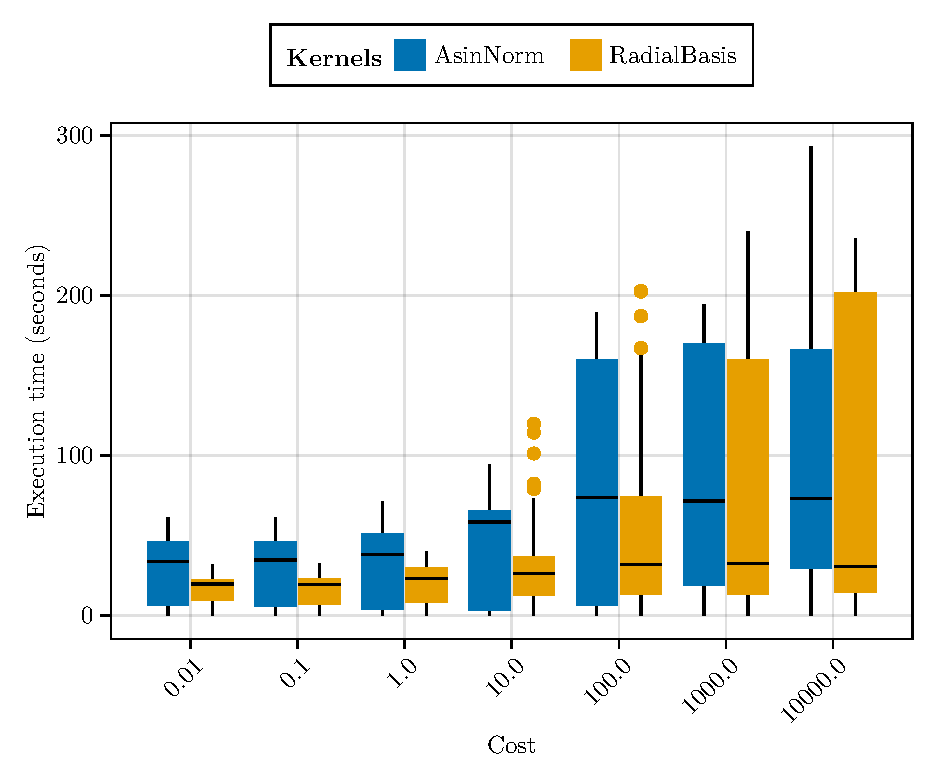
\includegraphics[width=0.6\textwidth]{plots/exec_cost}
    \caption{Time by cost parameter for normalized arcsine kernel on CompActs dataset}
    \label{fig:time-asinnorm-scaled-compacts}
\end{figure}

We can see that the cost hyperparameter has a significant effect on the
computational cost of both kernels. However, there is still a lot of variation
which comes from the effect of other hyperparameters, the data and even the
environment in which the experiments were run.

Instead, we can compute the ``speedup'' of the normalized arcsine kernel
in relation to the RBF kernel. That is, the ratio between the time taken
by the RBF kernel and the normalized arcsine kernel:
\begin{equation}
    \text{speedup} = \frac{T_{\text{RBF}}}{T_{\text{Asin}}} \label{eq:speedup}
\end{equation}
if the speedup is greater than 1, it means that the normalized arcsine kernel
is faster than the RBF kernel. If it is less than 1, it means that the RBF
kernel is faster than the normalized arcsine kernel. Since there are a lot
of outliers, we use the median instead of the mean to compute the speedup. We
do so by taking the median execution time for configuration of dataset, kernel,
and hyperparameters across all folds and values of sigma and gamma and computing
the speedup using \cref{eq:speedup} for each one. Averaging these speedups
gives us a speedup of $0.68$, which means that the RBF kernel is faster by
a factor of $1/0.68 = 1.47$.
